 [262~r\textsuperscript{o}] \rule[-4mm]{0mm}{10mm}$\displaystyle \frac{a^2}{a - \sqrt{\vphantom{2ax}} 2ax} \, \sqcap \, y$.
sumatur ejus loco
\begin{wrapfigure}[7]{l}{0.27\textwidth}
   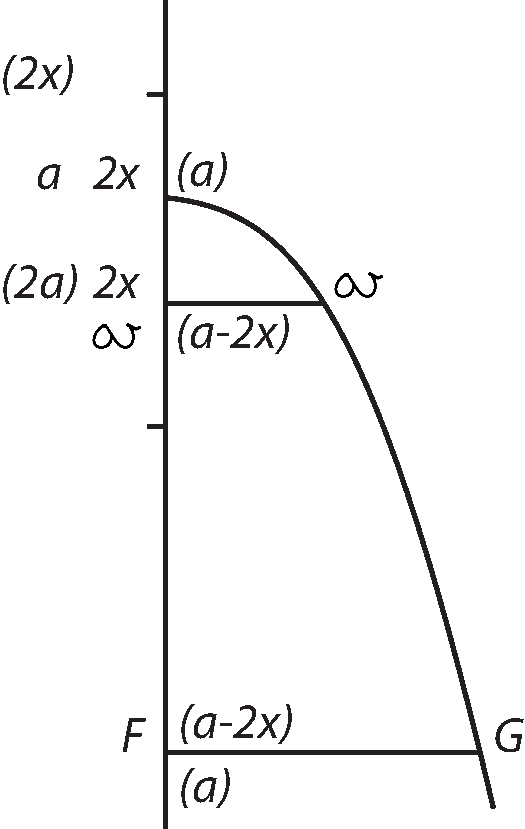
\includegraphics[trim = 0mm 0mm -10mm 0mm, clip, width=0.27\textwidth]{images/lh0351303_262r-d1.pdf}
     \center[\textit{Fig. 2}] % \caption{Bildbeschreibung}
    \end{wrapfigure} 
\rule[-4mm]{0mm}{10mm}$\displaystyle \frac{a \sqrt{\vphantom{2ax}} 2ax}{a - \sqrt{\vphantom{2ax}} 2ax} \, \sqcap \, \pi$. 
et fiet dividendo:
\edtext{$\displaystyle \protect \rule[-4mm]{0mm}{10mm} \pi \, \sqcap \, \sqrt{\protect \vphantom{2ax}} 2ax + 2ax + 2ax \sqrt{\protect \vphantom{2ax}} 2ax + 4a^2x^2 + 2a^2x^2 \sqrt{\protect \vphantom{2ax}} 2ax$ etc.}{\lemma{$\displaystyle \pi \, \sqcap \, \sqrt{\protect \vphantom{2ax}} 2ax + 2ax + 2ax \sqrt{\protect \vphantom{2ax}} 2ax + 4a^2x^2 + 2a^2x^2 \sqrt{\protect \vphantom{2ax}} 2ax$ etc.}\Cfootnote{Die Reihenentwicklung ist fehlerhaft. Der korrekte Ausdruck lautet:
$\displaystyle \pi = 2ax + 2x + \frac{2x \sqrt{2ax}}{a} + \frac{4x^2}{a} + \frac{4x^2 \sqrt{2ax}}{a^2} + \frac{8x^3}{a^2} + \frac{8x^3 \sqrt{2ax}}{a^3} + \frac{16x^4}{a^3} + \frac{16x^4 \sqrt{2ax}}{a^4} + \frac{32x^5}{a^4} + \cdots$
Der Fehler beeinflusst den weiteren Verlauf der Rechnung bis zum falschen Ergebnis:
$\displaystyle \dsig = \frac{\sqrt{2ax}}{a-2ax}$.
Richtig hei{\ss}t es:
$\displaystyle \dsig = \frac{a \sqrt{2ax}}{a - 2x}$.}}
\rule[-4mm]{0mm}{10mm}adeoque excerpendo rationales et irrationales separatim, erit
\rule[-4mm]{0mm}{10mm}$\displaystyle \pi \, \sqcap \, 2ax + 4a^2x^2 + 8a^3x^3 \, \mbox{etc.} \, \sqcap \, \frac{2ax}{a-2ax}$. 
quae est ad Hyperbolam,
\rule[-4mm]{0mm}{10mm}$\displaystyle \sqrt{\vphantom{2ax}} 2ax + 2ax \sqrt{\vphantom{2ax}} 2ax + 4ax^2 
%
%Zeile10
% 
\sqrt{\vphantom{2ax}} 2ax \ \mbox{etc.} \, \sqcap \, \frac{\sqrt{\vphantom{2ax}} 2ax}{a-2ax} \, \sqcap \, \dsig$
\edtext{quae ideo etiam pendet ex hyperbola}{\lemma{}\Bfootnote{quae [...] hyperbola \textit{erg.} \textit{L}}}. Jam
\rule[-4mm]{0mm}{10mm}$\displaystyle \frac{\sqrt{\vphantom{2ax}} 2ax}{a-2ax} \, \sqcap \, \dsig$. 
pro $\displaystyle a-2x$ ponendo $\displaystyle z$, fiet
$\displaystyle 2ax \ \sqcap \ a^2 - az$
adeoque:
\rule[-4mm]{0mm}{10mm}\edtext{$\displaystyle \frac{\sqrt{a^2 - az}}{z} \, \sqcap \, \protect \dsig$.}
{\lemma{$\displaystyle \frac{\sqrt{a^2 - az}}{z} \, \sqcap \, ??§$}
\Cfootnote{Substitutionsergebnis im Nenner falsch, da Leibniz $z = a - 2x$, nicht $z = a - 2ax$ substituiert hat.}}
Jam momentum ipsarum $\displaystyle \dsig$ ex 
%
%neue Seite
%
basi $\displaystyle FG \, \sqcap \, \sqrt{\vphantom{2ax}}2ax$ seu \rule[-4mm]{0mm}{10mm}$\displaystyle \sqrt{a^2 - a[z]}$\edtext{}{\Bfootnote{$\displaystyle \sqrt{a^2 - ax}$ \textit{\ L \"{a}ndert Hrsg.}}}
ad parabolam
$\displaystyle y^2a^2 - 2a^3y + a^4 \, \sqcap \ 2ay^2x$
pone
\rule[-4mm]{0mm}{10mm}\edtext{$\displaystyle x \, \sqcap \, z + \frac{a}{2}$.}
{\lemma{$\displaystyle x \, \sqcap \, z + \frac{a}{2}$}
\Cfootnote{Gelten $\displaystyle z = a - 2x$ und $z = x - \frac{a}{2}$, so muss $a = 2x$ sein. Dieser Fall ist in der senkrechten Koordinatenachse von [\textit{Fig. 2}] angedeutet. Weitere Fehler folgen. Das richtige Ergebnis f\"{u}r $\displaystyle y$ lautet:
$\displaystyle y = \frac{- \, a^2 \pm \sqrt{a^4 + 2a^3z}}{2z}$.}}
fiet:
\rule[-4mm]{0mm}{10mm}$\displaystyle \ovalbox{$y^2a^2$} \, - 2a^3y + a^4 \, \sqcap \ 2ay^2z \ \ovalbox{$\! +\, y^2a^2$}$
adeoque
$\displaystyle z \, \sqcap \, [-] \, \frac{a^2}{y} + \frac{a^3}{2y^2}$\edtext{.}{\lemma{}\Bfootnote{\textit{\ L \"{a}ndert Hrsg.}}}
item:
\rule[-4mm]{0mm}{10mm}\edtext{$\displaystyle y^2 + \frac{a^2}{z} y + \frac{a^4}{4z^2} \, \sqcap \, a^4 + \frac{a^4}{4z^2}$.
}{\lemma{$\displaystyle y^2 + \frac{a^2}{z} y + \frac{a^4}{4z^2} \, \sqcap \, a^4 + \frac{a^4}{4z^2}$}
\Cfootnote{Die Gleichung ist falsch abgeleitet. Statt $\displaystyle a^4$ muss es dort heißen: $\displaystyle \frac{a^3}{2z}$. Der Fehler wirkt sich auf den weiteren Verlauf der Rechnungen bis auf $\displaystyle \theta$ aus.}}et
\rule[-4mm]{0mm}{10mm}$\displaystyle y + \frac{a^2}{2z} \, \sqcap \, \frac{a \sqrt{z^2 + a^2}}{z}$.
Ergo quaerendae omnes:
\rule[-4mm]{0mm}{10mm}$\displaystyle \frac{\sqrt{z^2 + a^2}}{z} \, \sqcap \, \theta$.
quae proinde etiam redeunt ad hyperbolam.
\pend
%
%Zeile 5
%
\pstart
Hactenus de resistentia absoluta\protect\index{Sachverzeichnis}{resistentia absoluta}. \\
\pend
\pstart
\centering[\textit{Teil 2}]
\pend
\pstart
\noindent\edtext{La resistence des surfaces des corps au mouuement d'autres corps est ou absolue, et independante de la vitesse du corps meu, ou respective, c'est \`{a} dire d'autant plus grande 
%
%Zeile 10
%
que le corps meu va plus viste. J'ay trouu\'{e} que la raison des temps aux espaces dans un mouuement, diminu\'{e} par la resistance absolue ne peut estre [expliqu\'{e}e]\edtext{}{\Bfootnote{expliqu\'{e}\textit{\ L \"{a}ndert Hrsg.}}} que par le moyen des Logarithmes, soit qu'on suppose}{\lemma{}\Bfootnote{\textit{(1)}\ Resistentiam absolutam comperi redire ad Logarithmos \textit{(2)}\  La Resistence  \textit{(a)}\ absolue  \textit{(b)}\ des surfaces  \textit{(c)}\ que les corps trouuent \`{a} rouler ou \`{a} glisser sur des surfaces  \textit{(aa)}\ polies  \textit{(bb)}\ dures d'autres corps, \textit{(3)}\  La resistence  \textit{(a)}\ absolue  \textit{(b)}\ des  \textit{(aa)}\ corps  \textit{(bb)}\ surfaces [...] est  \textbar\ ou \textit{erg.}\ \textbar\  absolue,   \textit{(aaa)}\ ou  \textit{(bbb)}\ c'est \`{a} dire  \textit{(ccc)}\ et independante [...] trouu\'{e}  \textit{(aaaa)}\ que la resistance absolue revient aux logarithmes, soit qu'on suppose  \textit{(bbbb)}\ que la raison [...] absolue  \textit{(aaaaa)}\ revient aux  \textit{(bbbbb)}\ ne peut [...] suppose \textit{L}}} une diminution uniforme de la vitesse, en chaque endroit par o\`{u} le mobile passe, comme j'ay demonstr\'{e} dans un \edtext{cahier,}{\lemma{cahier}\Cfootnote{Vgl. vermutlich N. 5\textsubscript{3} und 5\textsubscript{4}.}} que j'avois donn\'{e} \`{a} part, soit qu'on suppose que la vistesse se diminue en raison soubsdouble des espaces, 
%
%Zeile 15
%
comme il s'ensuit necessairement en supposant que le mobile surmonte en chaque endroit de \edtext{l'espace certains ressorts egaux, entre eux qui}{\lemma{l'espace}\Bfootnote{ \textit{(1)}\ des ressorts \textit{(2)}\ certains ressorts egaux,  \textit{(a)}\ pour passer entre  \textit{(b)}\ qui  \textit{(c)}\ entre eux qui \textit{L}}} s'opposoient \`{a} son passage, pour veu qu'on fasse abstraction de la matiere \edtext{ou du poids}{\lemma{ou}\Bfootnote{\textit{(1)}\ pesanteur \textit{(2)}\ du poids \textit{L}}} m\^{e}me de ces petits ressorts. Mais comme leur matiere \edtext{ou moles}{\lemma{}\Bfootnote{ou moles \textit{erg.} \textit{L}}} ne semble pas tout \`{a} fait \`{a} negliger, quelque petite qu'elle puisse estre,%\pend